\documentclass[a4paper]{article}
\usepackage{tikz}
\usetikzlibrary{shapes.geometric, shadows}

\begin{document}

\section*{TikZ-Beispiel: Platzierung von Nodes}

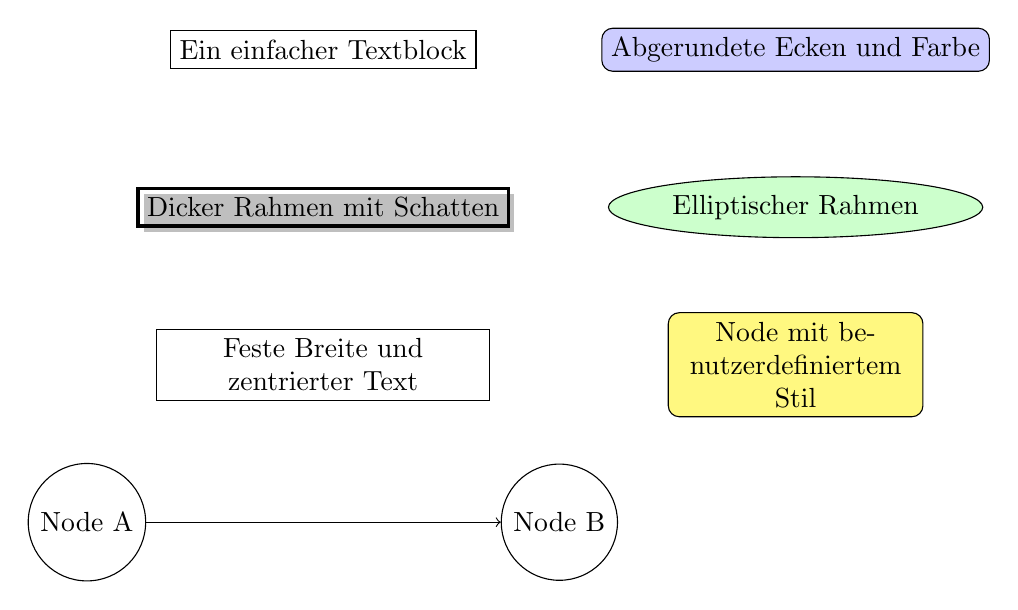
\begin{tikzpicture}

% 1. Ein einfacher Node mit Text und einem Rechteckrahmen
\node[draw] at (0, 0) {Ein einfacher Textblock};

% 2. Node mit abgerundeten Ecken und Hintergrundfarbe
\node[draw, rounded corners, fill=blue!20] at (6, 0) {Abgerundete Ecken und Farbe};

% 3. Node mit dickem Rahmen und Schatten
\node[draw, very thick, drop shadow] at (0, -2) {Dicker Rahmen mit Schatten};

% 4. Node mit geometrischer Form (Ellipse)
\node[draw, ellipse, fill=green!20] at (6, -2) {Elliptischer Rahmen};

% 5. Node mit fester Breite und zentriertem Text
\node[draw, text width=4cm, align=center] at (0, -4) {Feste Breite und zentrierter Text};

% 6. Node mit benutzerdefiniertem Stil
\tikzset{customstyle/.style={draw, fill=yellow!50, text width=3cm, align=center, rounded corners}}
\node[customstyle] at (6, -4) {Node mit benutzerdefiniertem Stil};

% 7. Zwei Nodes mit Verbindungslinie
\node[draw, circle] (node1) at (-3, -6) {Node A};
\node[draw, circle] (node2) at (3, -6) {Node B};
\draw[->] (node1) -- (node2);

\end{tikzpicture}

\end{document}
